% !TeX root = ../main.tex
% Add the above to each chapter to make compiling the PDF easier in some editors.

\chapter{Introduction}\label{chapter:introduction}

Computer vision has been an important role in the automation of processes in many different areas. A well-studied subject within the field of computer vision is humans. In detecting and tracking humans, humans are usually localized, by means of bounding boxes, within a single or multiple views. In pose estimation, a human body is usually represented, by a skeleton composed of a set of joints. The objective in pose estimation is to recover the joint locations of human bodies in 2D images or 3D space. While 2D single person detection and tracking of humans has been well addressed in real-world environments, 3D multi-person pose estimation remains an open problem, due to the complex scenarios that it has to consider. In this thesis, we study the problem from multiple views. We investigate the approach that aggregates multiple view information using epiporlar geometry. Our ultimate goal is to estimate 3D human pose from multiple 2D views.

\section{Motivation}
Estimation 3D multi-person human poses have been addressed, by using a single view \cite{singleshotmultiperson2018, LCR2019, iskakov2019learnable} or multi-view camera \cite{multiviewpose, 20204DAssociation, voxelpose, 20163DPictorial, dong2019fast, Chen_2020_CVPR}. Regardless of single view or multi-view approaches, the first step is usually generating 2D likelihood maps of joint locations by a backbone network trained on a 2D pose estimation task. However, the accuracy of the 2D pose estimation backbone degrades significantly when joints being occluded \cite{Sarandi18IROSW}, resulting single-view methods to produce unrealistic 3D poses. Since occlusions are a common issue in multi-person and in-the-wild environments, leveraging multi-view information becomes a natural choice in 3D multi-person pose estimation. Some previous studies adopt 3D pictorial structure (3DPS) \cite{20163DPictorial, multiviewpose, 20204DAssociation}, where the 3D poses are recovered from 2D joints in a discretized 3-space, with predefined geometric constraint of human bodies. However, a severe problem of 3DPS is the expensive computational cost due to the huge state space with multiple people in multiple views. Other approaches rely on deep networks that operate on volumetric grids \cite{voxelpose, iskakov2019learnable} to combine features coming from different views in accordance with epipolar geometry. Unfortunately, it requires a discretized space that covers the whole environment, which is memory demanding and, more importantly, impractical in outdoor environments.



\section{Problem Definition and Challenges}
In this work, we address the 3D multi-person pose estimation task from multiple views using epipolar geometry. Inspired by the lightweight approaches that utilize multiview geometry \cite{multiviewpose, epipolartransformers, zhang2020adafuse}, we use a lightweight 2D pose estimator trained on the COCO dataset as backbone and aggregate multi-view information using epipolar geometry. Our goal is to automatically estimate the pose of multiple individuals in 3D space, given a set of images from a calibrated multi-view camera system.  However, the transition from 2D to 3D space and from single to multiple human pose estimation is a challenging task.

\begin{figure}[htpb]
	\centering
	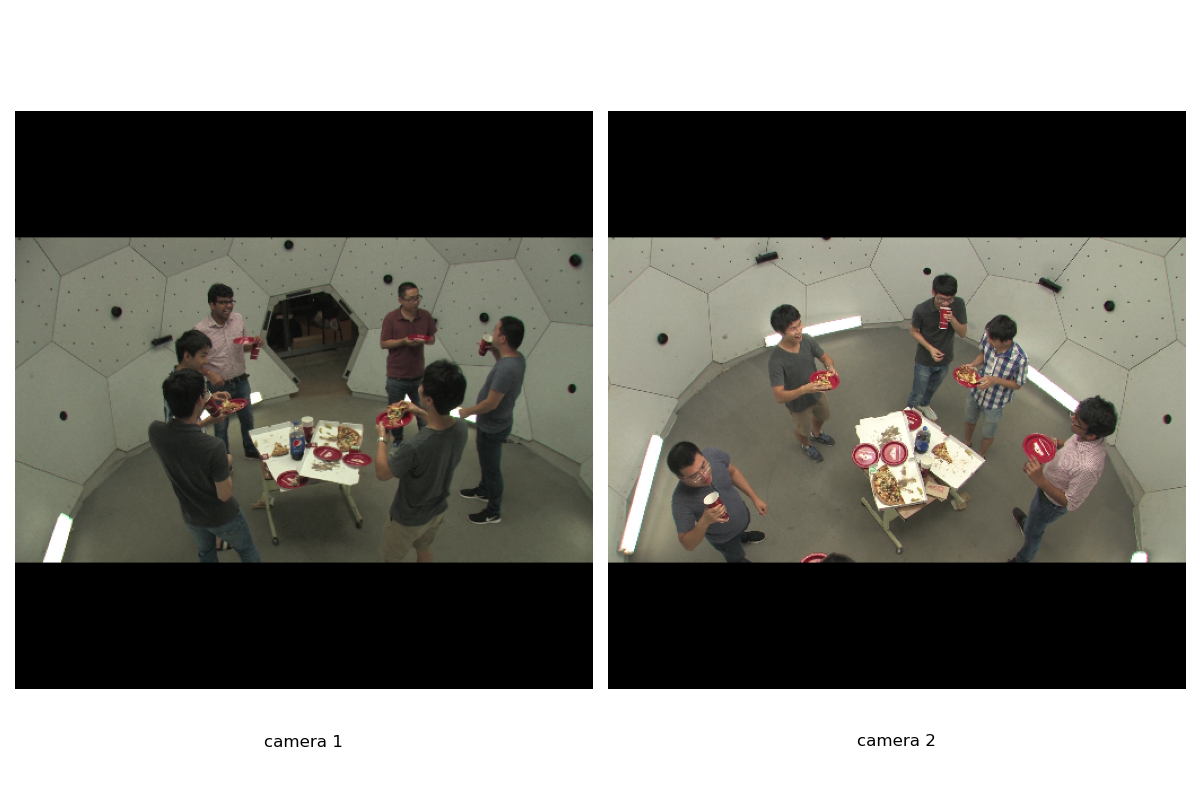
\includegraphics[width=0.7\columnwidth]{figures/ch1/Figure_1.png}
	\caption{Estimating multi-person 3D human poses without using computational heavy operations is the task we address in this work.}
	\label{fig:ch1-multiview-occlusion}
\end{figure}

\begin{figure}[htpb]
	\centering
	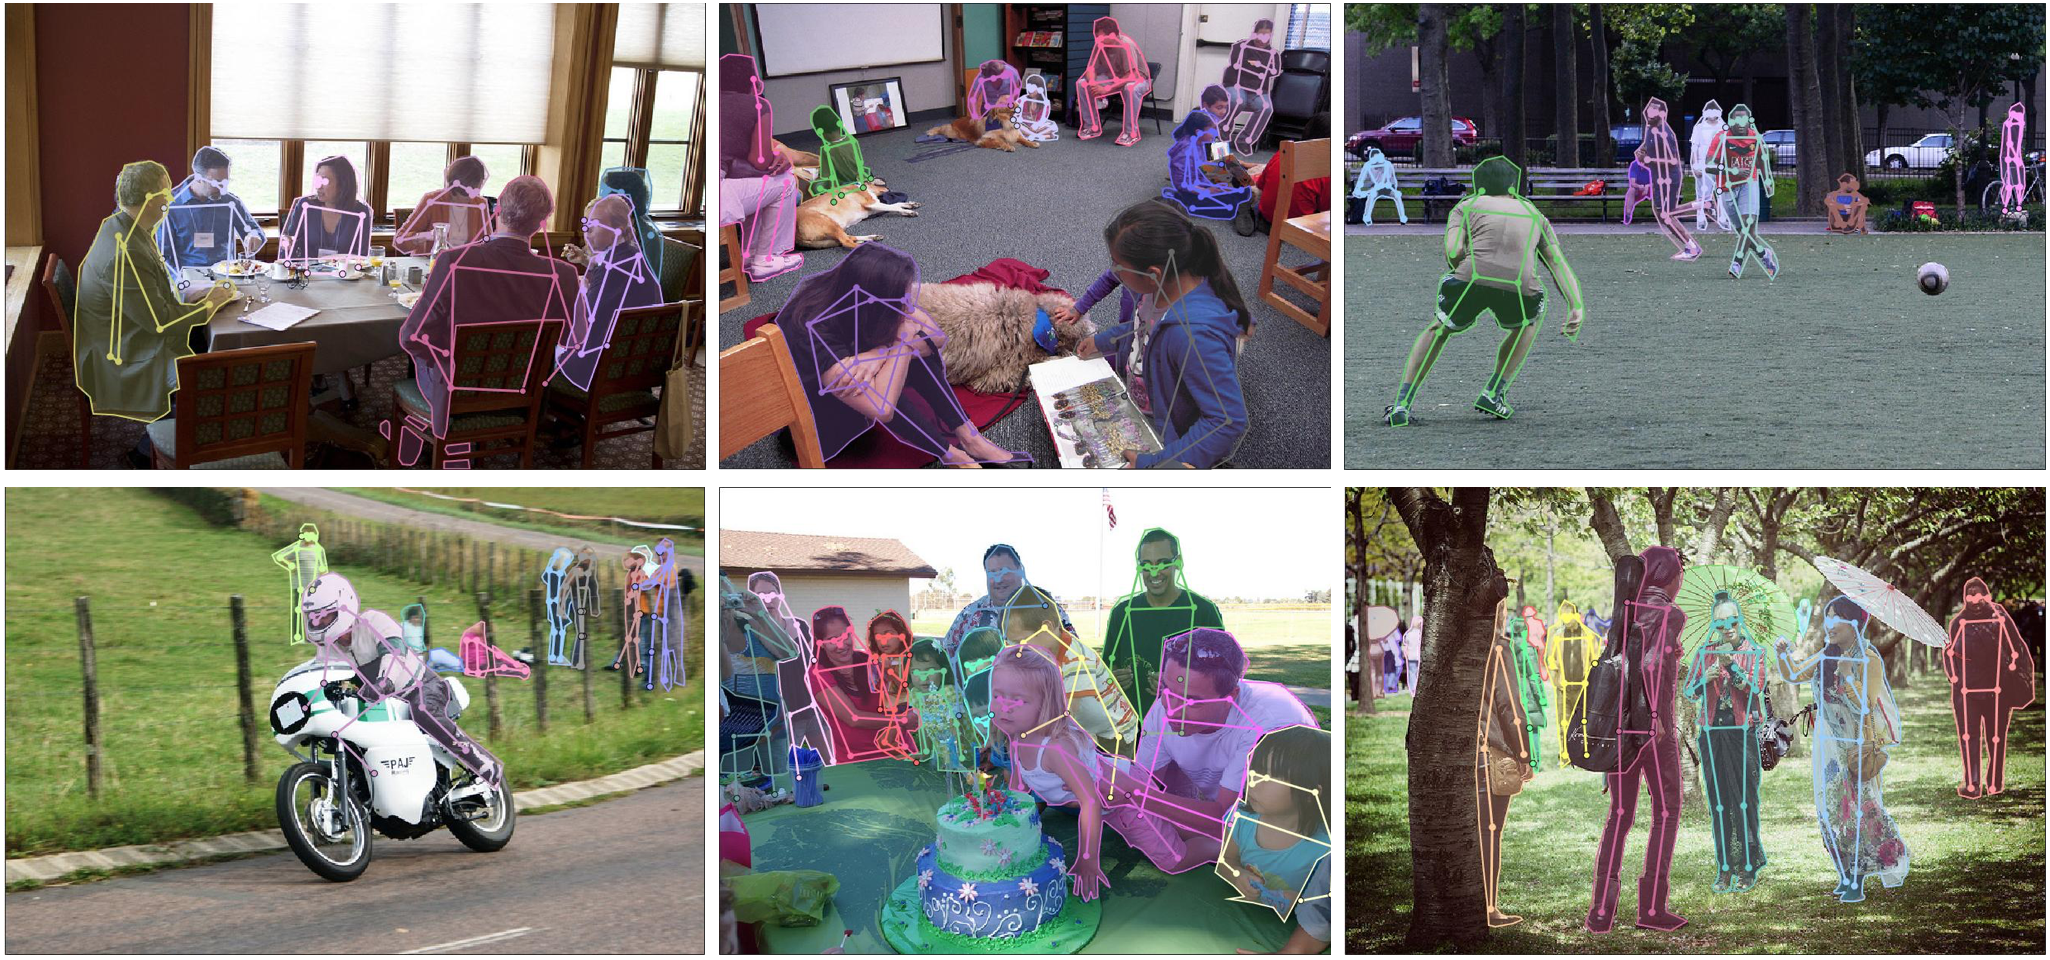
\includegraphics[width=0.7\columnwidth]{figures/ch1/coco-dataset.png}
	\caption{A human pose is approximated by a rigid skeletons, composed by various joints. Performing human pose estimation, however, from images can be a difficult task due to the body pose and appearance high variation.}
	\label{fig:ch1-coco-dataset}
\end{figure}

First of all, learning 2D human bodies from image data is a hard task due to its articulation and large deformation it can go through. Thus, 2D human pose estimation researchers usually use a rigid skeleton compose of a various number of joints, such as elbow, pelvis, etc., shown in \ref{fig:ch1-coco-dataset}. Since the 2D models are built from images, we have to compensate the missing dimension when estimating 3D poses. 

Secondly, the appearance of a joint varies significantly from one view to another. Most 2D human pose datasets that based on natural images provide only frontal and horizontal views. Yet it is common in multi-person environments that most of the joints are occluded in frontal view and can only be revealed at a novel view, see Fig.\ref{fig:ch1-multiview-occlusion}. Occlusions cause a serious problem in 2D multi-person human pose estimation in single view images \cite{Sarandi18IROSW}; occlusions can not only caused by objects but by oneself and other humans as well, shown in Fig. \ref{fig:ch1-multiview-occlusion}.

Moreover, recent works \cite{20204DAssociation, multiviewpose, dong2019fast, 20143DPictorial} cast multi-person 3D human poses estimation as associating 2D poses in all camera views. This is complicated problem in multiple human 3D pose estimation when the identity of individuals is unknown. An association between the individuals across all views is required to avoid mixing the body parts of different individuals. For instance, a left hand of one person in one view will have multiple left hand candidates in other camera views coming not only from the same person, but also from other individuals and potential false positive detections. In practice, this will create incorrect body part hypotheses that can lead to fake body poses in the 3D space. In addition, matching 2D poses between all pairs of views still makes the computational complexity explode as the number of cameras increases \cite{Chen_2020_CVPR} . 

To address these challenges, we propose to fuse features from multiple views using epipolar geometry and a deep convolution network. Our intuition is that a joint that being occluded in one view could be visible in other views and a deep convolution network can learn how to see through occlusions from the fused features.

\section{Applications}
A framework for multi-person human pose estimation from multiple views has a wide range applications, such as motion capture, surveillance, sports, and human activity recognition, etc.. We provide some examples that our framework could be applied on. Motion capture systems haven been beneficial in film industry, especially for CG characters. The current technology for estimating reliable 3D human poses is based on maker-based solutions, which work only in a studio environment. On the contrary, our approach is marker-less and can be adapted to any unconstrained environments. Another useful scenario for our framework is sport science or analysis, where athletes can not wear MOCAP suits. For example, estimating the poses of basketball players, captured from different view, supports game analysis. In addition, body pose estimation can be used to study the tactic of opponents or to improve the training of teams. Furthermore, our framework can be used in the public surveillance systems since there are usually multiple cameras installed in public areas. As this work was done during the COVID-19 pandemic period, a crowd control system, combining our work and activity recognition, for detecting citizen gathering in a large group would be beneficial to the health of public. Lastly, our frame work can be applied on multi-pedestrian path prediction for autonomous driving. Lastly, our frame can add to human action recognition, where human poses are one of the strong cues.
In general, our frame benefits various real-world applications because it is less computation demanding and suits for unconstraint environments. 

\section{Thesis Outline}
We provide an overview for each chapter of the thesis
\begin{description}
  \item[$\bullet$ Chapter 2] \noindent We present the theoretical background of our work. 
  \item[$\bullet$ Chapter 3] \noindent In this chapter, we provide an overview of the current researches in the field of 3D human pose estimation and compare the \noindent difference between our work and related researches.  
  \item[$\bullet$ Chapter 4] \noindent We explain the design of our feature fusion modules and the network architectures.  
  \item[$\bullet$ Chapter 5] \noindent In this chapter, we give an overlook of two different datasets we used in this work and explain metrics being used by the datasets to evaluate the performance of our model. Futher, we introduce the data augmentation methods. 
  \item[$\bullet$ Chapter 6] \noindent We evaluate the performance of our work and give an ablation study
  \item[$\bullet$ Chapter 7] \noindent We conclude our work by presenting our findings, the limitations
of the proposed methods and our directions for future work.
\end{description}



